%File: smile2_aaai2026.tex
\documentclass[letterpaper]{article} % DO NOT CHANGE THIS
\usepackage[submission]{aaai2026}  % DO NOT CHANGE THIS
\usepackage{times}  % DO NOT CHANGE THIS
\usepackage{helvet}  % DO NOT CHANGE THIS
\usepackage{courier}  % DO NOT CHANGE THIS
\usepackage[hyphens]{url}  % DO NOT CHANGE THIS
\usepackage{graphicx} % DO NOT CHANGE THIS
\urlstyle{rm} % DO NOT CHANGE THIS
\def\UrlFont{\rm}  % DO NOT CHANGE THIS
\usepackage{natbib}  % DO NOT CHANGE THIS AND DO NOT ADD ANY OPTIONS TO IT
\usepackage{caption} % DO NOT CHANGE THIS AND DO NOT ADD ANY OPTIONS TO IT
\frenchspacing  % DO NOT CHANGE THIS
\setlength{\pdfpagewidth}{8.5in} % DO NOT CHANGE THIS
\setlength{\pdfpageheight}{11in} % DO NOT CHANGE THIS
\usepackage{amsmath,amssymb,amsfonts,bm}
\usepackage{mathtools}
\usepackage{booktabs}
\usepackage{makecell}
\usepackage{adjustbox}
\usepackage[table]{xcolor}
\pdfinfo{
/TemplateVersion (2026.1)
}

\setcounter{secnumdepth}{0}
\graphicspath{{figures/}}

\newcommand{\smiletwo}{SMILE\textsuperscript{2}}
\newcommand{\sfestimator}{\textsc{SFEstimator}}
\newcommand{\sfe}{\textsc{SFE}}
\newcommand{\sfevolver}{\textsc{SFEvolver}}
\newcommand{\swp}{\textsc{SWP}}
\newcommand{\Cs}{\mathrm{Cs}}
\newcommand{\Sn}{\mathrm{Sn}}
\definecolor{compareorange}{RGB}{255,250,244}
\definecolor{oursgreen}{RGB}{229,246,232}
\definecolor{costgray}{RGB}{250,250,250}

\title{SMILE\textsuperscript{2}: Spectral Modulated Imaging via Learned Estimation--Evolution for Snapshot Compressive Hyperspectral Reconstruction}
\author{Anonymous Submission}
\affiliations{Paper ID: Anonymous}

\begin{document}
\maketitle

\begin{abstract}
Coded aperture snapshot spectral imaging (CASSI) aims to recover a three-dimensional hyperspectral image from a single two-dimensional coded measurement, resulting in a severely under-determined spatial--spectral inverse problem.
Recent end-to-end CNN and Transformer models have greatly improved reconstruction quality by learning spatial--spectral mappings, but their central interaction mechanisms are still largely implemented as generic convolutional transformations or implicit token mixing.
Consequently, how information should propagate over the hyperspectral \((x,y,\lambda)\) field remains weakly structured and difficult to interpret.
In this paper, we propose \smiletwo{}, a single-pass spectral-field estimation--evolution framework for end-to-end CASSI reconstruction.
Instead of directly mapping an aliased shift-back field to the output cube, \smiletwo{} first estimates an initial spectral field from measurement-consistent cues and then evolves it with a unified spatial--spectral physical operator.
The core component is the Spectral Wave Propagator (\swp{}), which adapts a three-dimensional damped wave equation to the discretely sampled HSI field and performs global propagation through a Fourier-domain closed-form solution with \(O(N\log N)\) operator-level complexity.
Together with CASSI preparation, \sfestimator{}, and \sfevolver{}, \swp{} forms a compact estimation--evolution reconstructor.
On the TSA simulation benchmark and real CASSI measurements, \smiletwo{} achieves state-of-the-art end-to-end reconstruction quality under compact computation.
In particular, \smiletwo-L reaches 37.07 dB PSNR and 0.965 SSIM with 3.19M parameters and 38.60G FLOPs, while obtaining favorable spectral angle mapper (SAM) fidelity among reproducible end-to-end baselines.
\end{abstract}

\section{Introduction}

Hyperspectral images (HSIs) record spectral responses over a dense wavelength axis in addition to two spatial dimensions.
They therefore provide material and scene information that is unavailable in ordinary RGB imaging.
Conventional spectral imaging systems usually scan either spatial positions or wavelengths, which limits acquisition speed.
Coded aperture snapshot spectral imaging (CASSI) uses a coded aperture and a dispersive element to compress a three-dimensional HSI cube into a single two-dimensional measurement, enabling efficient snapshot spectral acquisition \cite{wagadarikar2008cassi,gehm2007ddcassi}.
This optical efficiency comes with a difficult inverse problem: a single measurement \(Y\) must recover a spatial--spectral field \(X\in\mathbb{R}^{H\times W\times L}\).

\begin{figure}[!t]
  \centering
  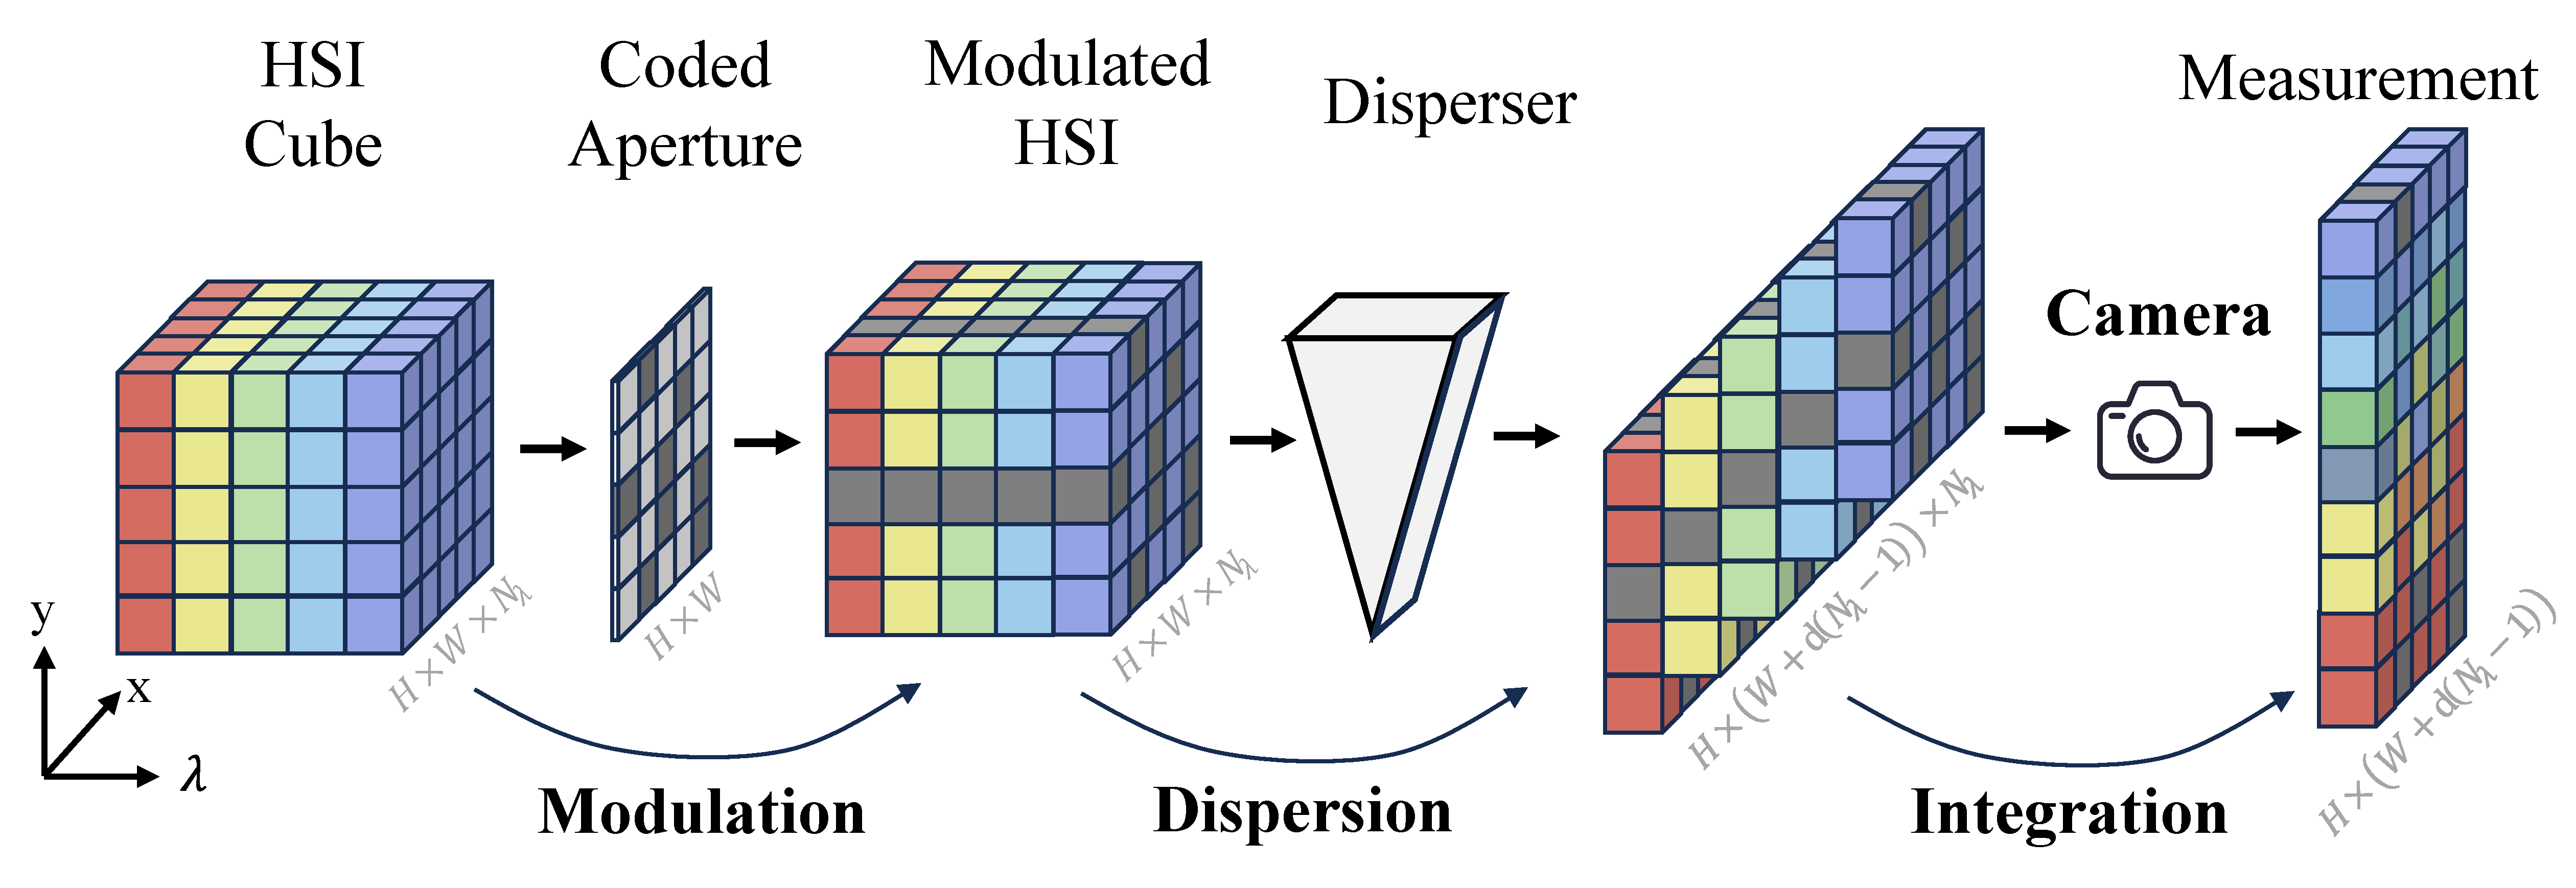
\includegraphics[width=\columnwidth]{final/0CASSI_tight.pdf}
  \caption{CASSI forward imaging. A spectral cube \(X\) is modulated by the coded aperture \(M\), dispersed into shifted spectral measurements, and compressed into a single measurement \(Y=\Phi X\).}
  \label{fig:cassi_forward}
\end{figure}

Unlike RGB image restoration, CASSI reconstruction must recover both intensity and spectral direction.
We view the HSI as a sampled spatial--spectral field over the discrete \((x,y,\lambda)\) grid, rather than as independent two-dimensional bands.
This field view does not assume arbitrary continuous-coordinate querying; instead, it provides a mathematical interface for jointly describing second-order spatial and spectral structures.
Existing CASSI networks have empirically exploited such spatial--spectral redundancy through convolution, recurrent modeling, and spectral attention \cite{miao2019lambdanet,meng2020tsanet,cai2022mst,cai2022cst,cai2022mstpp}.
The same observation is also consistent with classical hyperspectral unmixing, where spectra of natural materials often lie in a low-dimensional and correlated subspace \cite{bioucasdias2012unmixing}.
More broadly, recent discussions on a scientific theory of deep learning suggest that mathematical structures and dynamical descriptions can provide useful ways to understand deep models \cite{simon2026scientifictheorydeeplearning}, while physics-guided machine learning demonstrates the value of embedding scientific structure into neural operators \cite{karniadakis2021piml,willard2022scientificknowledge,weinan2017dynamicalsystems}.
This work explores such a direction for CASSI reconstruction.

Most end-to-end CASSI methods directly learn the mapping from \(Y\) to \(X\), relying on convolutions, recurrent modules, or attention to enlarge the spatial--spectral receptive field.
Attention is a powerful universal interaction mechanism, but its all-to-all token mixing does not explicitly state how spectral information propagates over the \(x,y,\lambda\) field, and global pairwise interactions are expensive at large resolutions \cite{vaswani2017attention,liu2021swin}.
Meanwhile, the CASSI forward model itself provides valuable physical cues.
The mask, dispersion, shift-back operation, and normalization map reveal how the 2D measurement is multiplexed from the 3D spectral cube.
Model-driven and hybrid end-to-end methods have shown that using \(\Phi\), \(\Phi^\top\), and mask coverage can help reduce aliasing and ambiguity \cite{meng2020gapnet,huang2021dgsmp}.
However, these cues are often used as initialization or correction features before the subsequent network again relies on generic learned mixing.

This observation is important because the shift-back field \(H_0\) is not a clean HSI estimate.
It preserves coarse scene structures, but each location is still affected by coded-mask modulation, overlapped shifted spectra, nonuniform sensing coverage, and residual measurement inconsistency.
Directly feeding this dirty spectral field into a generic token mixer leaves the roles of correction and propagation entangled.
A more structured single-pass alternative is to first estimate a cleaner initial spectral field from measurement-consistent cues, and then evolve this field through a spatial--spectral operator whose propagation behavior is explicitly parameterized.
This motivates the central question:

\begin{quote}
\centering
\textit{Can CASSI reconstruction be formulated as initial spectral-field estimation followed by evolution through a unified spatial--spectral physical operator?}
\end{quote}

We answer this question with \smiletwo{}, a single-pass estimation--evolution framework.
First, \swp{} adapts a 3D damped wave equation to the CASSI spatial--spectral field, uses Fourier-domain closed-form evolution over \(f_x,f_y,f_\lambda\), and gates the wave field by the shifted sensing mask \(\Phi_s\).
Second, CASSI preparation constructs the shift-back field \(H_0\), normalization map \(P\), and residual-adjoint cue \(Q_0\) from the forward model.
Third, \sfestimator{} estimates an initial spectral field \(U_1\) from \([H_0,Q_0,M,H_0\odot M]\), while \sfevolver{} further propagates it to obtain the final reconstruction \(\hat X\).
Compared with the \(O(N^2)\) pairwise token mixing of self-attention, \swp{} provides global interaction through an \(O(N\log N)\) Fourier-domain operator.

Our contributions are summarized as follows.
\begin{itemize}
  \item We propose a single-pass spectral-field estimation--evolution framework for CASSI, explicitly formulating end-to-end reconstruction as initial spectral-field estimation followed by Fourier-domain physical evolution.
  \item We design \swp{}, a mask-gated damped-wave propagation operator that performs structured global spatial--spectral mixing through a closed-form wave kernel.
  \item We build compact SMILE-S/M/L variants and obtain state-of-the-art end-to-end reconstruction quality on the TSA simulation benchmark, with favorable SAM and visual fidelity.
  \item We provide non-black-box evidence, including cross-band mixing and equal-count occlusion analysis, to explain how \smiletwo{} exploits spectral context.
\end{itemize}

\section{Related Work}

\subsection{End-to-End CASSI Reconstruction}

Early CASSI reconstruction methods rely on optimization and hand-crafted priors, such as GAP-TV, TwIST, and DeSCI \cite{yuan2016gaptv,bioucasdias2007twist,liu2018rank}.
These methods are interpretable but limited in reconstruction quality and efficiency.
Deep networks transform CASSI reconstruction into a data-driven mapping.
\(\lambda\)-Net, TSA-Net, GAP-Net, and HDNet improve reconstruction through end-to-end regression, spatial--spectral self-attention, physical operator embedding, and dual-domain learning, respectively \cite{miao2019lambdanet,meng2020tsanet,meng2020gapnet,hu2022hdnet}.
Transformer-based models further strengthen long-range spectral modeling.
MST introduces spectral-wise self-attention, while CST and MST++ improve the efficiency of spectral interaction through sparse and multi-stage designs \cite{cai2022mst,cai2022cst,cai2022mstpp}.
Recent end-to-end models also explore lightweight sensing, self-supervised adaptation, and spatial/spectral frequency modeling \cite{cai2023bisci,zeng2024sahsci,liu2025ssfan}.
Overall, end-to-end CASSI models are efficient and effective, but their global spatial--spectral interaction is usually expressed by generic learned mixing rather than by an explicit propagation process.

\subsection{Forward-Model Cues in End-to-End Reconstruction}

Although end-to-end networks learn a direct mapping from measurement to HSI, the CASSI forward model remains essential for network design.
GAP-Net embeds projection and back-projection into the network, and DGSMP constructs deep priors from the sensing matrix structure \cite{meng2020gapnet,huang2021dgsmp}.
These works show that the sensing operator, shifted mask, and measurement-adjoint cues provide useful initialization and correction information.
Multi-stage unfolding methods further exploit the forward model through repeated data-consistency and learned-prior updates, often achieving higher absolute PSNR at higher iterative cost \cite{cai2022dauhst,zhang2024dpu,zhang2024ssr}.
\smiletwo{} builds on the broader insight that forward-model cues matter in a single-pass end-to-end framework. CASSI preparation condenses measurement-aware cues into \(H_0\), \(P\), and \(Q_0\), enabling \sfestimator{} and \sfevolver{} to perform field correction and propagation within one feed-forward reconstruction process.

\subsection{Frequency- and PDE-Inspired Vision Modeling}

Frequency-domain modeling offers a different route to global interaction.
Fourier Neural Operator learns solution operators in function spaces and demonstrates that Fourier modes can efficiently parameterize global mappings \cite{li2021fno}.
FNet mixes tokens with Fourier transforms, GFNet learns global filters, and AFNO adapts neural operator ideas to high-resolution vision features \cite{leethorp2022fnet,rao2021gfnet,guibas2022afno}.
In image restoration, FFTformer and frequency-modulated restoration networks use Fourier-domain attention or frequency modulation to model degradation-related components \cite{kong2023fftformer,cui2024csnet}.
These studies indicate that frequency transforms can provide global receptive fields without explicitly constructing quadratic token affinities.

Another related direction is PDE-inspired vision modeling.
vHeat builds vision models upon heat conduction, while WaveFormer uses a wave equation to design frequency-time decoupled visual modeling \cite{wang2024vheat,shu2026waveformer}.
Compared with total variation, which mainly constrains local first-order gradients, and compared with heat diffusion, which is biased toward smoothing, a damped wave equation contains propagation, oscillation, and damping.
This makes it suitable for modeling second-order spatial--spectral structures and frequency-selective attenuation.
In spectral reconstruction, Phy-CoSF introduces physics-guided continuous spectral fields for snapshot compressive imaging reconstruction and super-resolution \cite{chen2026phycosf}.
However, these frequency- and PDE-inspired works do not directly address CASSI-specific mask modulation, wavelength-dependent shift, 2D-to-3D compression, and shift-back initialization.
\smiletwo{} differs by coupling CASSI preparation with a mask-gated damped-wave spectral-field propagator in a fixed-grid, single-pass CASSI reconstruction framework.

\begin{figure*}[!t]
  \centering
  \fbox{\rule{0pt}{1.75in}\rule{0.94\textwidth}{0pt}}
  \caption{Conceptual overview of the transition from attention mixing to physical evolution. \smiletwo{} replaces generic pairwise token interaction with structured spatial--spectral propagation governed by a Fourier-domain damped-wave kernel.}
  \label{fig:overall}
\end{figure*}

\section{Method}

\subsection{Spectral-Field Formulation and Notation}

Let \(X\in\mathbb{R}^{H\times W\times L}\) denote the target HSI, where the axes correspond to \(x\), \(y\), and wavelength \(\lambda\).
Let \(Y\in\mathbb{R}^{H\times W'}\) denote the 2D CASSI measurement and \(M\in\mathbb{R}^{H\times W\times L}\) the unshifted coded mask.
The complete sensing operator is denoted by \(\Phi\), which includes mask modulation, spectral shift, and spectral summation.
The shifted mask stack induced by CASSI shifts is denoted by \(\Phi_s\); its measurement-domain energy gives the normalization map \(P=\Phi\Phi^\top\), and its field-aligned slices are used as \swp{} gates.
The shift-back field, residual-adjoint cue, estimated spectral field, and final reconstruction are denoted by \(H_0\), \(Q_0\), \(U_1\), and \(U_2=\hat X\), respectively.
We use \(\epsilon\) as a small positive constant for numerical stability and gate lower bounds.

\subsection{CASSI Forward Model and Field Preparation}

The CASSI measurement is obtained by band-wise coding, wavelength-dependent shifting, and spectral summation:
\begin{equation}
Y=\Phi X=\sum_{\lambda=1}^{L}\mathrm{Shift}_{\lambda}(M_\lambda\odot X_\lambda).
\label{eq:cassi_forward}
\end{equation}
The normalization map is
\begin{equation}
P=\Phi\Phi^\top=\sum_{\lambda=1}^{L}\Phi_{s,\lambda}^{2}.
\label{eq:normalization}
\end{equation}
In vectorized notation, \(\Phi\) maps a 3D spectral field to the 2D measurement plane; hence \(\Phi\Phi^\top\) corresponds to a diagonal normalization operator in the measurement domain.
In implementation, the full matrix is not stored.
Instead, \(P\in\mathbb{R}^{H\times W'}\) is represented by its diagonal map, which summarizes the shifted mask energy contributing to each measurement pixel.
For a binary mask, \(P\) can be interpreted as the effective coding coverage at each measurement location.
It is therefore not a global scalar but a pixel-wise measurement-domain weight map.

We first construct a dirty shift-back field:
\begin{equation}
H_0=\mathcal{B}(Y),
\label{eq:h0}
\end{equation}
where \(\mathcal{B}\) copies each shifted measurement slice back to its spectral-channel coordinates with a fixed scale normalization.
\(H_0\) contains major scene structures but remains an aliased spectral field affected by mask modulation, dispersion overlap, and spectral ambiguity.
We further compute a residual-adjoint cue:
\begin{equation}
R_0=Y-\Phi H_0,\qquad
Q_0=\Phi^\top(R_0/(P+\epsilon)).
\label{eq:q0}
\end{equation}
The input to \sfestimator{} is
\begin{equation}
C_0=[H_0,Q_0,M,H_0\odot M].
\label{eq:c0}
\end{equation}
Here \(Q_0\) exposes the measurement residual left by the initial shift-back field, while \(H_0\odot M\) explicitly couples image content with the coded aperture.

\subsection{Spectral Wave Propagator}

\swp{} is the core physical evolution operator used in both \sfestimator{} and \sfevolver{}.
Given a spectral field \(z\in\mathbb{R}^{H\times W\times L}\), \swp{} regards it as a field over \((x,y,\lambda)\) and performs learnable damped-wave propagation.
The evolution time \(t\) denotes feature-field propagation depth, rather than exposure time or physical travel time in the CASSI optical path.
Thus, \swp{} is a physics-inspired regularized propagation operator for reconstruction, not a direct simulation of the optical hardware.

To condition propagation on the sensing process, \swp{} first gates the input field with the shifted sensing mask:
\begin{equation}
\tilde z=(\epsilon+(1-\epsilon)\Phi_s)\odot z.
\label{eq:mask_gate}
\end{equation}
Two lightweight learnable mappings then generate the initial displacement and velocity of the wave equation:
\begin{equation}
u_0=\Pi_u(\tilde z),\qquad
v_0=\Pi_v(\tilde z).
\label{eq:uv0_spatial}
\end{equation}
Applying a real-valued 3D Fourier transform over \(x,y,\lambda\) gives
\begin{equation}
\hat u_0=\mathcal{F}_{x,y,\lambda}(u_0),\qquad
\hat v_0=\mathcal{F}_{x,y,\lambda}(v_0).
\label{eq:uv0}
\end{equation}

The physical backbone of \swp{} is the anisotropic 3D damped wave equation:
\begin{equation}
\partial_{tt}u+\alpha\partial_tu
=v_s^2(\partial_{xx}+\partial_{yy})u+v_\lambda^2\partial_{\lambda\lambda}u.
\label{eq:wave_pde}
\end{equation}
For a Fourier mode \(\boldsymbol f=(f_x,f_y,f_\lambda)\), the second-order derivatives become multiplicative factors.
The PDE is converted into a per-mode second-order ordinary differential equation:
\begin{equation}
\frac{d^2\hat u(\boldsymbol f,t)}{dt^2}
+\alpha(f_\lambda)\frac{d\hat u(\boldsymbol f,t)}{dt}
+\omega_0^2(\boldsymbol f)\hat u(\boldsymbol f,t)=0,
\label{eq:mode_ode}
\end{equation}
where
\begin{align}
\omega_0^2(\boldsymbol f)
&=(2\pi)^2\left[
v_s^2(f_\lambda)(f_x^2+f_y^2)+v_\lambda^2 f_\lambda^2
\right], \nonumber\\
\eta(\boldsymbol f)&=\omega_0^2(\boldsymbol f)-\left(\frac{\alpha(f_\lambda)}{2}\right)^2 .
\label{eq:omega}
\end{align}
The closed-form evolution is
\begin{align}
\hat u(\boldsymbol f,t)=
&e^{-\alpha(f_\lambda)t/2}
\Big[
\hat u_0(\boldsymbol f)\Cs(\eta(\boldsymbol f),t) \nonumber\\
&+\left(\hat v_0(\boldsymbol f)
+\frac{\alpha(f_\lambda)}{2}\hat u_0(\boldsymbol f)\right)
\Sn(\eta(\boldsymbol f),t)
\Big].
\label{eq:closed_form}
\end{align}
\(\Cs\) and \(\Sn\) denote cosine-like and sine-like terms that unify under-damped and over-damped cases.
For \(\eta>0\), \(\Cs(\eta,t)=\cos(\sqrt{\eta}t)\) and \(\Sn(\eta,t)=\sin(\sqrt{\eta}t)/\sqrt{\eta}\); for \(\eta<0\), they naturally become hyperbolic functions.
The evolved field is obtained by inverse FFT:
\begin{equation}
u(t)=\mathcal{F}^{-1}_{x,y,\lambda}(\hat u(\boldsymbol f,t)).
\label{eq:ifft}
\end{equation}

The parameters \(\alpha(f_\lambda)\) and \(v_s(f_\lambda)\) are spectral-mode-dependent damping and propagation speed, while \(v_\lambda\) controls the strength of the spectral second derivative.
In the implemented \swp{} layers, \(\alpha\) and \(v_s\) are layer-specific learnable vectors indexed by the spectral-mode dimension, initialized as constant damping and speed values and mapped through a softplus function to keep them positive.
The scalar \(v_\lambda\) and the evolution depth \(t\) are also learned with the same positivity constraint.
The FFT along the \(\lambda\) axis uses a periodic discrete spectral-mode basis to expand the finite 28-band sequence.
This basis is used to parameterize spectral modes over the sampled HSI grid, without assuming that real spectral reflectance is physically periodic along wavelength.
Consequently, \(\alpha(f_\lambda)\) and \(v_s(f_\lambda)\) are treated as learnable parameters over the discrete spectral-mode basis.
The output of \swp{} is written as a residual update:
\begin{equation}
\mathcal{W}_\theta(z,\Phi_s)=z+\Pi_o(u(t)).
\label{eq:swp_residual}
\end{equation}
Self-attention explicitly computes pairwise token relations with \(O(N^2)\) core complexity.
\swp{} instead performs global propagation through FFT and a closed-form wave kernel, yielding \(O(N\log N)\) operator-level complexity.

\begin{figure*}[!t]
  \centering
  
\includegraphics[width=\textwidth]{final/2swap_tight.pdf}
  \caption{Overall architecture of \smiletwo{}. CASSI preparation constructs \(H_0\), \(Q_0\), and \(\Phi_s\) from the measurement and mask. \sfestimator{} estimates the initial spectral field \(U_1\), and \sfevolver{} evolves it into the final reconstruction \(U_2=\hat X\).}
  \label{fig:swapunet}
\end{figure*}

\subsection{Spectral Field Estimator}

The aliased shift-back field \(H_0\) is not directly suitable as the final reconstruction.
\sfestimator{} first predicts a zero-initialized residual correction:
\begin{equation}
\Delta_\psi(C_0)=
\mathrm{Conv}^{0}_{3\times3}
\left(
\sigma(\mathrm{Conv}_{3\times3}(C_0))
\right),
\label{eq:sfe_delta}
\end{equation}
where \(\mathrm{Conv}^{0}_{3\times3}\) denotes a zero-initialized \(3\times3\) convolution.
Therefore, at the beginning of training,
\begin{equation}
Z_0=H_0+\Delta_\psi(C_0)=H_0,
\label{eq:z0}
\end{equation}
so the network does not destroy the shift-back initialization.
The first SWP-based U-Net estimates a cleaner spectral field:
\begin{equation}
U_1=\mathcal{E}_{\theta_E}^{\mathrm{SWP}}(Z_0,\Phi_s).
\label{eq:u1}
\end{equation}
In the architecture, the SFE stem and the first SWP-based U-Net together constitute \sfestimator{}.

\subsection{Spectral Field Evolver}

\sfevolver{} does not recompute \(R_0\) or \(Q_0\).
Instead, it further evolves the estimated spectral field \(U_1\):
\begin{equation}
U_2=\mathcal{E}_{\theta_V}^{\mathrm{SWP}}(U_1,\Phi_s),\qquad
\hat X=U_2.
\label{eq:u2}
\end{equation}
The main signal flow is
\begin{equation}
Y,M \rightarrow H_0,Q_0,M,\Phi_s \rightarrow U_1 \rightarrow \hat X.
\label{eq:pipeline}
\end{equation}
We instantiate three compact variants to evaluate the same estimation--evolution design under different computational budgets: SMILE-S uses the compact \([2,2,2]\) backbone with partially tied estimator/evolver parameters, SMILE-M decouples the estimator and evolver parameters at the same width, and SMILE-L increases the U-Net width to \([2,4,4]\) for higher capacity.

\begin{figure*}[!t]
  \centering
  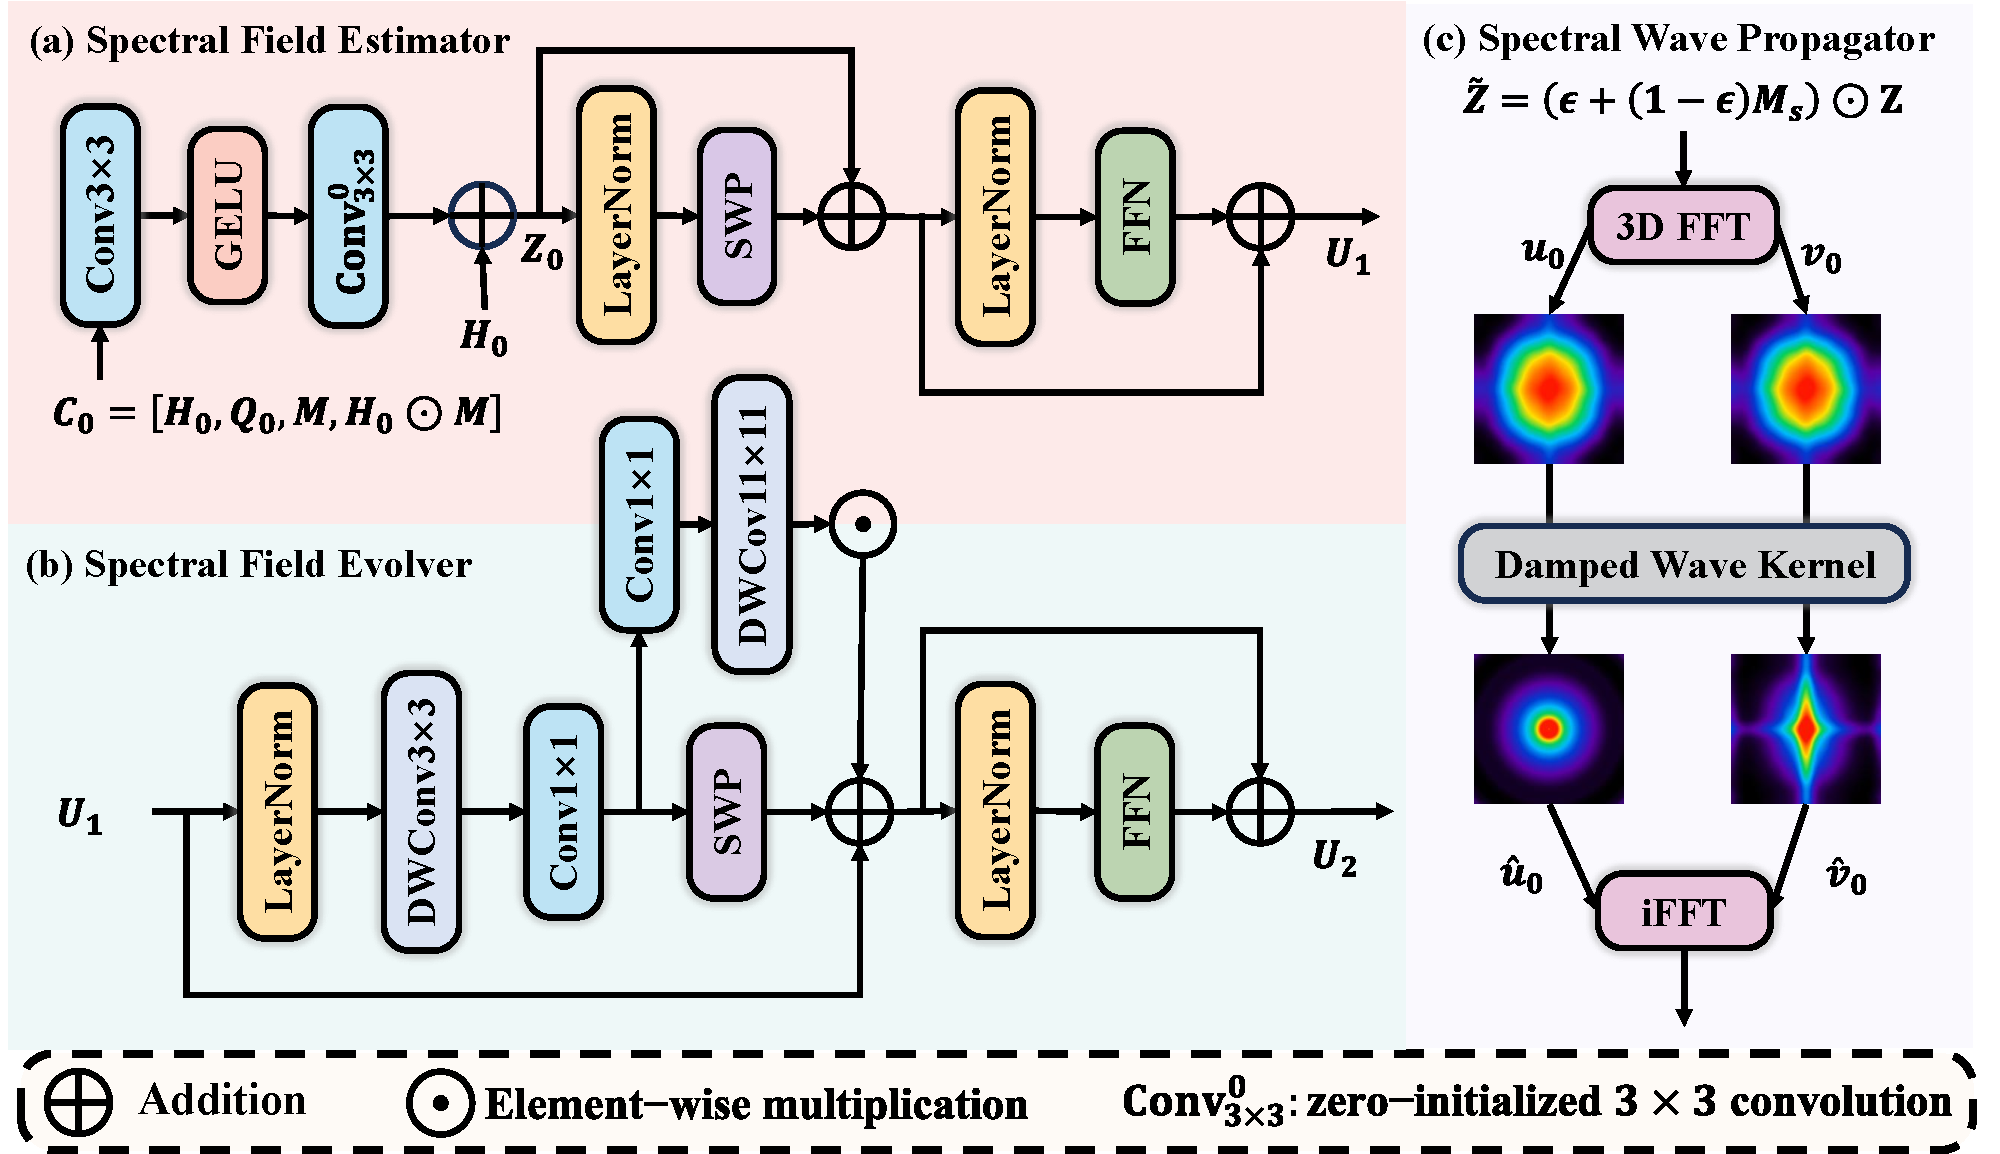
\includegraphics[width=0.95\textwidth]{final/3swp_tight.pdf}
  \caption{Signal flow of \sfestimator{}, \sfevolver{}, and the embedded \swp{} operator. The \swp{} branch performs mask-gated Fourier-domain damped-wave propagation, while \sfestimator{} and \sfevolver{} differ in their input fields and update roles.}
  \label{fig:swp}
\end{figure*}

\section{Experiments}

\subsection{Experimental Settings}

Simulation experiments are conducted on the TSA simulation benchmark with ten test scenes of spatial size \(256\times256\) and \(L=28\) spectral channels.
Training data are sampled from CAVE and KAIST hyperspectral datasets \cite{yasuma2010cave,choi2017kaist}.
We report PSNR, SSIM, and spectral angle mapper (SAM), where SAM measures spectral directional error and is important for hyperspectral fidelity \cite{kruse1993sam}.
All training and evaluation experiments are conducted on NVIDIA A800 GPUs with 80GB memory.
The main models are trained for 300 epochs with Adam and cosine learning-rate decay.

\sfestimator{} and \sfevolver{} output \(U_1\) and \(U_2=\hat X\), respectively.
Training uses only weighted RMSE reconstruction supervision:
\begin{equation}
\mathcal{L}_{\mathrm{train}}
=\sum_{k=1}^{2}\beta_k\,\mathrm{RMSE}(U_k,X),
\qquad
\boldsymbol{\beta}=[0.2,1.0].
\label{eq:train_loss_sfe}
\end{equation}
The objective does not include auxiliary SAM/SSIM, spectral-derivative, spectral-angle, or explicit \(\|\Phi\hat X-Y\|\) data-fidelity losses.
Forward-model consistency enters before reconstruction through CASSI preparation: \(H_0\) supplies the dirty shift-back field, \(Q_0\) exposes the normalized residual-adjoint cue, and \(P\) represents the measurement-domain coding coverage.

\subsection{Quantitative Comparison}

Table~\ref{tab:sota_main} reports per-scene results on the TSA simulation benchmark.
For methods with released weights or reproducible official implementations, we evaluate them under the same protocol; for methods without released weights or reconstructed outputs, PSNR/SSIM are taken from the corresponding papers and SAM is denoted by ``--''.
Compared with earlier CNN and Transformer E2E baselines, \smiletwo{} consistently improves reconstruction quality while keeping the model compact.
\smiletwo-M uses 2.00M parameters and 28.28G FLOPs, reaching 36.57 dB PSNR, 0.961 SSIM, and 0.097 rad SAM.
Scaling the same estimation--evolution principle to \smiletwo-L improves the average score to 37.07 dB PSNR, 0.965 SSIM, and 0.086 rad SAM with 3.19M parameters and 38.60G FLOPs.
These results indicate that structured spectral-field evolution can serve as an effective E2E reconstruction prior, improving both image-level fidelity and spectral-angle consistency.

\begin{table*}[!t]
\centering
\caption{Quantitative comparison on the TSA simulation benchmark. Each scene cell reports PSNR, SSIM, and SAM(rad) from top to bottom. Methods with public checkpoints or official reproducible implementations are evaluated under the same protocol; for methods without released weights or reconstructed outputs, PSNR/SSIM are taken from the corresponding papers and SAM is unavailable.}
\label{tab:sota_main}
\scriptsize
\setlength{\tabcolsep}{3.0pt}
\renewcommand{\arraystretch}{1.03}
\resizebox{0.98\textwidth}{!}{
\begin{tabular}{ll|cc|*{10}{c}|c}
\toprule
Algorithm & Method & Params & GFLOPs & S1 & S2 & S3 & S4 & S5 & S6 & S7 & S8 & S9 & S10 & Avg \\
\midrule
\rowcolor{costgray}
Optimization & TwIST~\cite{bioucasdias2007twist} & -- & -- & \makecell{25.16\\0.700\\--} & \makecell{23.02\\0.604\\--} & \makecell{21.40\\0.711\\--} & \makecell{30.19\\0.851\\--} & \makecell{21.41\\0.635\\--} & \makecell{20.95\\0.644\\--} & \makecell{22.20\\0.643\\--} & \makecell{21.82\\0.650\\--} & \makecell{22.42\\0.690\\--} & \makecell{22.67\\0.569\\--} & \makecell{23.12\\0.669\\--} \\
\rowcolor{costgray}
Optimization & GAP-TV~\cite{yuan2016gaptv} & 4.27 & 75.63 & \makecell{21.26\\0.490\\0.553} & \makecell{21.90\\0.578\\0.618} & \makecell{18.97\\0.506\\0.561} & \makecell{27.97\\0.794\\0.455} & \makecell{17.43\\0.429\\0.504} & \makecell{21.88\\0.688\\0.548} & \makecell{20.65\\0.442\\0.530} & \makecell{22.19\\0.700\\0.580} & \makecell{22.27\\0.609\\0.366} & \makecell{19.94\\0.615\\0.594} & \makecell{21.44\\0.585\\0.531} \\
\rowcolor{costgray}
Optimization & DeSCI~\cite{liu2018rank} & -- & -- & \makecell{27.13\\0.748\\--} & \makecell{23.04\\0.620\\--} & \makecell{26.62\\0.818\\--} & \makecell{34.96\\0.897\\--} & \makecell{23.94\\0.706\\--} & \makecell{22.38\\0.683\\--} & \makecell{24.45\\0.743\\--} & \makecell{22.03\\0.673\\--} & \makecell{24.56\\0.732\\--} & \makecell{23.59\\0.587\\--} & \makecell{25.27\\0.721\\--} \\
\rowcolor{costgray}
CNN & $\lambda$-Net~\cite{miao2019lambdanet} & 32.73 & 28.40 & \makecell{29.71\\0.832\\0.244} & \makecell{27.70\\0.746\\0.295} & \makecell{29.55\\0.852\\0.260} & \makecell{37.58\\0.919\\0.392} & \makecell{26.61\\0.804\\0.260} & \makecell{27.28\\0.809\\0.403} & \makecell{26.62\\0.783\\0.244} & \makecell{26.23\\0.807\\0.416} & \makecell{28.56\\0.805\\0.265} & \makecell{26.16\\0.723\\0.391} & \makecell{28.60\\0.808\\0.317} \\
\rowcolor{costgray}
CNN & TSA-Net~\cite{meng2020tsanet} & 44.25 & 73.83 & \makecell{24.42\\0.714\\0.256} & \makecell{23.38\\0.660\\0.315} & \makecell{17.30\\0.614\\0.445} & \makecell{26.34\\0.795\\0.415} & \makecell{20.51\\0.600\\0.275} & \makecell{22.29\\0.742\\0.368} & \makecell{21.35\\0.636\\0.374} & \makecell{22.25\\0.762\\0.395} & \makecell{20.27\\0.672\\0.446} & \makecell{21.29\\0.694\\0.442} & \makecell{21.94\\0.689\\0.373} \\
\rowcolor{costgray}
MAP+CNN & DGSMP~\cite{huang2021dgsmp} & 3.76 & 646.36 & \makecell{33.35\\0.920\\0.161} & \makecell{31.66\\0.892\\0.208} & \makecell{32.92\\0.925\\0.135} & \makecell{40.39\\0.970\\0.135} & \makecell{29.46\\0.894\\0.172} & \makecell{32.74\\0.938\\0.144} & \makecell{31.14\\0.898\\0.141} & \makecell{31.33\\0.932\\0.190} & \makecell{31.53\\0.925\\0.145} & \makecell{31.51\\0.934\\0.129} & \makecell{32.60\\0.923\\0.156} \\
\rowcolor{costgray}
CNN & HDNet~\cite{hu2022hdnet} & 2.37 & 154.73 & \makecell{35.11\\0.940\\0.129} & \makecell{35.65\\0.943\\0.142} & \makecell{36.05\\0.948\\0.099} & \makecell{42.48\\0.978\\0.101} & \makecell{32.67\\0.950\\0.089} & \makecell{34.47\\0.956\\0.120} & \makecell{33.64\\0.930\\0.114} & \makecell{32.45\\0.948\\0.141} & \makecell{34.85\\0.947\\0.110} & \makecell{32.34\\0.943\\0.119} & \makecell{34.97\\0.948\\0.116} \\
\rowcolor{compareorange}
Transformer & MST-L~\cite{cai2022mst} & 2.02 & 25.67 & \makecell{35.44\\0.946\\0.123} & \makecell{36.12\\0.949\\0.142} & \makecell{36.39\\0.955\\0.106} & \makecell{42.05\\0.977\\0.128} & \makecell{32.94\\0.950\\0.101} & \makecell{34.71\\0.957\\0.137} & \makecell{34.08\\0.932\\0.110} & \makecell{32.90\\0.953\\0.179} & \makecell{35.04\\0.947\\0.128} & \makecell{32.74\\0.946\\0.146} & \makecell{35.24\\0.951\\0.130} \\
\rowcolor{compareorange}
Transformer & CST-L~\cite{cai2022cst} & 3.00 & 20.34 & \makecell{35.82\\0.951\\0.116} & \makecell{36.52\\0.955\\0.118} & \makecell{37.45\\0.963\\0.082} & \makecell{42.46\\0.979\\0.100} & \makecell{33.34\\0.956\\0.078} & \makecell{35.48\\0.966\\0.104} & \makecell{34.40\\0.940\\0.098} & \makecell{33.80\\0.965\\0.119} & \makecell{35.88\\0.957\\0.100} & \makecell{33.35\\0.955\\0.103} & \makecell{35.85\\0.959\\0.102} \\
\rowcolor{compareorange}
Transformer & S2Transformer~\cite{wang2025s2transformer} & 1.80 & 27.21 & \makecell{36.17\\0.949\\--} & \makecell{37.57\\0.958\\--} & \makecell{37.29\\0.957\\--} & \makecell{42.96\\0.975\\--} & \makecell{34.40\\0.960\\--} & \makecell{36.44\\0.965\\--} & \makecell{35.41\\0.946\\--} & \makecell{34.50\\0.962\\--} & \makecell{36.54\\0.959\\--} & \makecell{33.57\\0.952\\--} & \makecell{36.48\\0.958\\--} \\
\rowcolor{compareorange}
Transformer & DSMT~\cite{luo2025dsmt} & 12.40 & 44.94 & \makecell{36.38\\0.958\\--} & \makecell{37.86\\0.965\\--} & \makecell{39.18\\0.968\\--} & \makecell{43.89\\0.985\\--} & \makecell{34.03\\0.965\\--} & \makecell{36.48\\0.972\\--} & \makecell{35.48\\0.952\\--} & \makecell{34.54\\0.969\\--} & \makecell{37.67\\0.966\\--} & \makecell{33.71\\0.959\\--} & \makecell{36.92\\0.966\\--} \\
\rowcolor{oursgreen}
Wave equation & \smiletwo-S & 1.02 & 28.28 & \makecell{35.68\\0.946\\0.114} & \makecell{36.39\\0.950\\0.131} & \makecell{37.39\\0.961\\0.084} & \makecell{44.07\\0.984\\0.104} & \makecell{33.42\\0.955\\0.086} & \makecell{35.20\\0.961\\0.123} & \makecell{34.29\\0.936\\0.101} & \makecell{33.27\\0.957\\0.148} & \makecell{37.21\\0.960\\0.102} & \makecell{32.45\\0.947\\0.124} & \makecell{35.94\\0.956\\0.112} \\
\rowcolor{oursgreen}
Wave equation & \smiletwo-M & 2.00 & 28.28 & \makecell{36.16\\0.952\\0.106} & \makecell{37.43\\0.959\\0.113} & \makecell{38.77\\0.967\\0.070} & \makecell{43.67\\0.982\\0.089} & \makecell{33.86\\0.960\\0.074} & \makecell{35.66\\0.965\\0.106} & \makecell{35.13\\0.947\\0.090} & \makecell{33.98\\0.964\\0.128} & \makecell{37.93\\0.965\\0.089} & \makecell{33.09\\0.953\\0.104} & \makecell{36.57\\0.961\\0.097} \\
\rowcolor{oursgreen}
Wave equation & \smiletwo-L & 3.19 & 38.60 & \makecell{36.60\\0.957\\0.091} & \makecell{38.04\\0.966\\0.097} & \makecell{39.25\\0.969\\0.071} & \makecell{44.78\\0.987\\0.080} & \makecell{34.23\\0.964\\0.072} & \makecell{35.94\\0.969\\0.089} & \makecell{35.61\\0.952\\0.078} & \makecell{33.96\\0.966\\0.103} & \makecell{38.65\\0.969\\0.082} & \makecell{33.59\\0.956\\0.097} & \makecell{37.07\\0.965\\0.086} \\
\bottomrule
\end{tabular}}
\end{table*}

\subsection{Qualitative Results}

\begin{figure*}[!t]
  \centering
  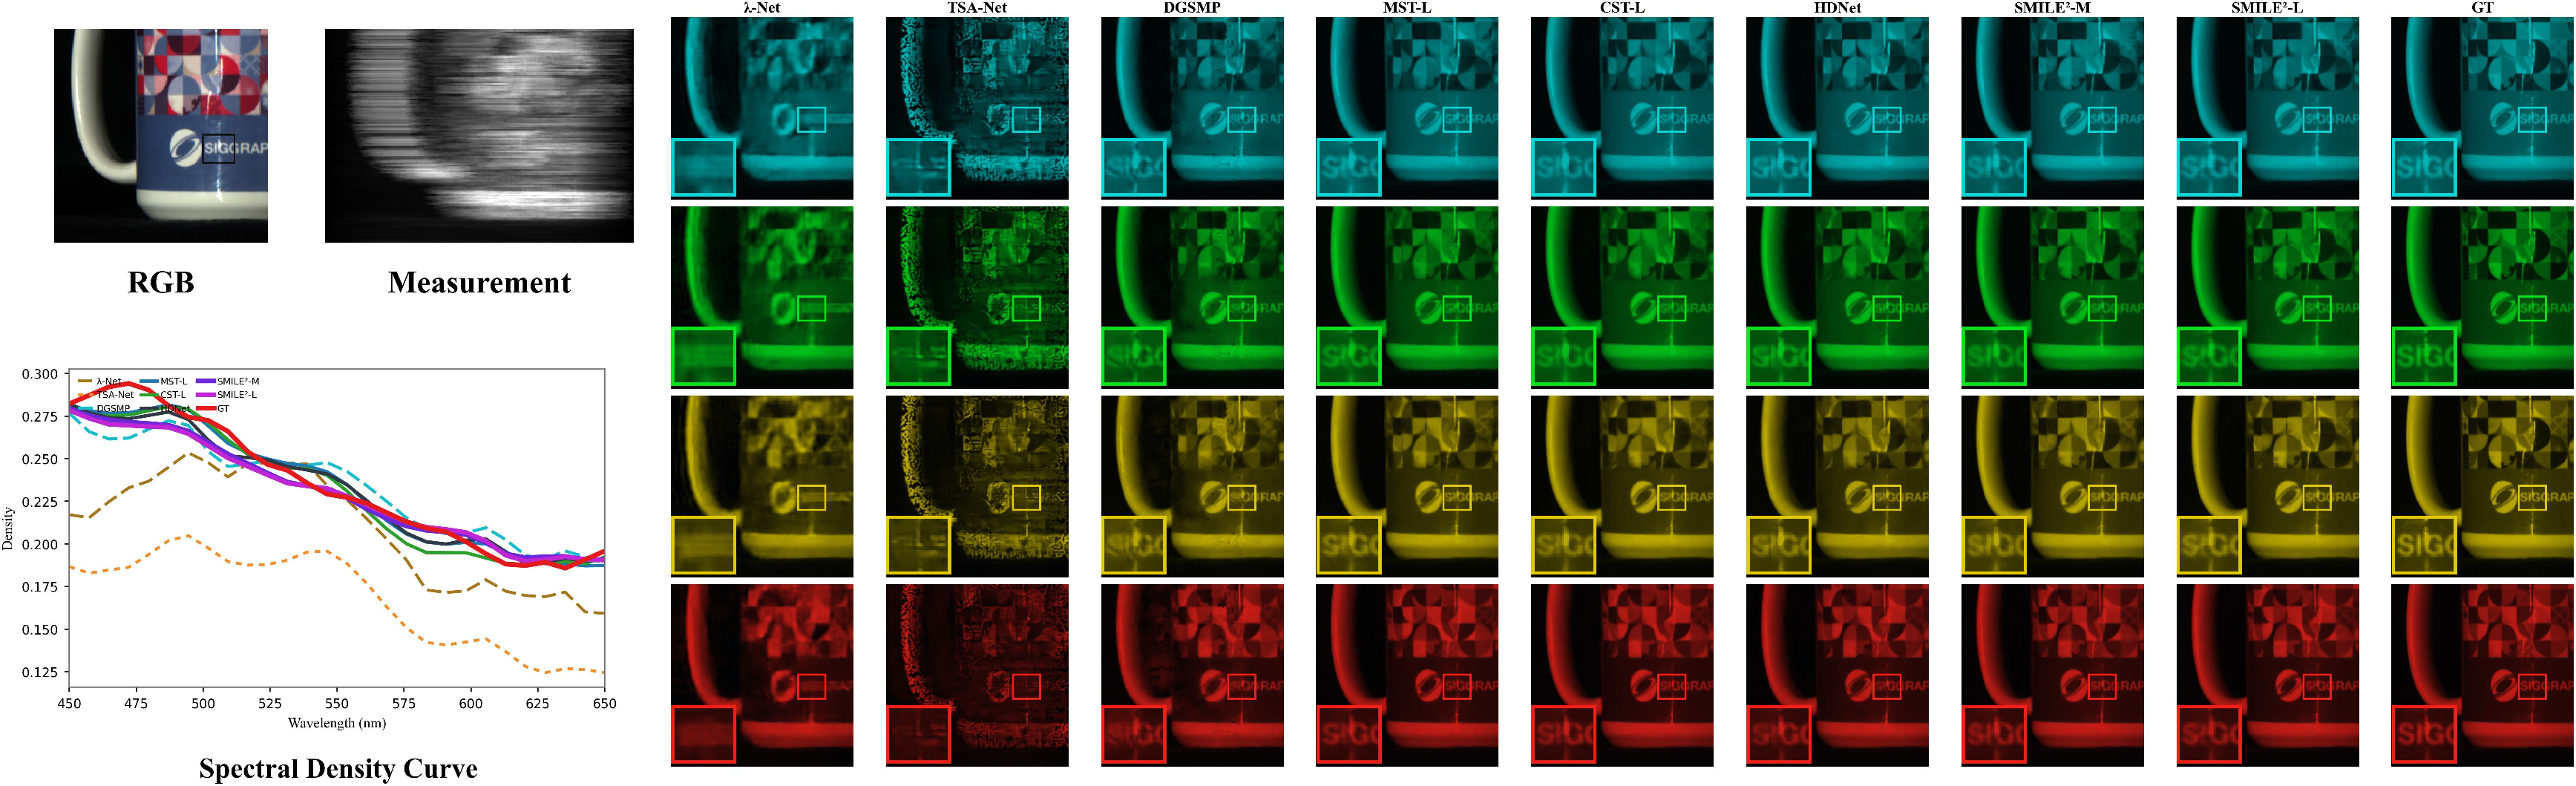
\includegraphics[width=\textwidth]{final/scene05_unified_layout.pdf}
  \caption{Simulation Scene 5. The figure compares RGB/measurement inputs, representative spectral bands, zoomed local regions, and spectral density curves.}
  \label{fig:sota_simu_scene5}
\end{figure*}

\begin{figure*}[!t]
  \centering
  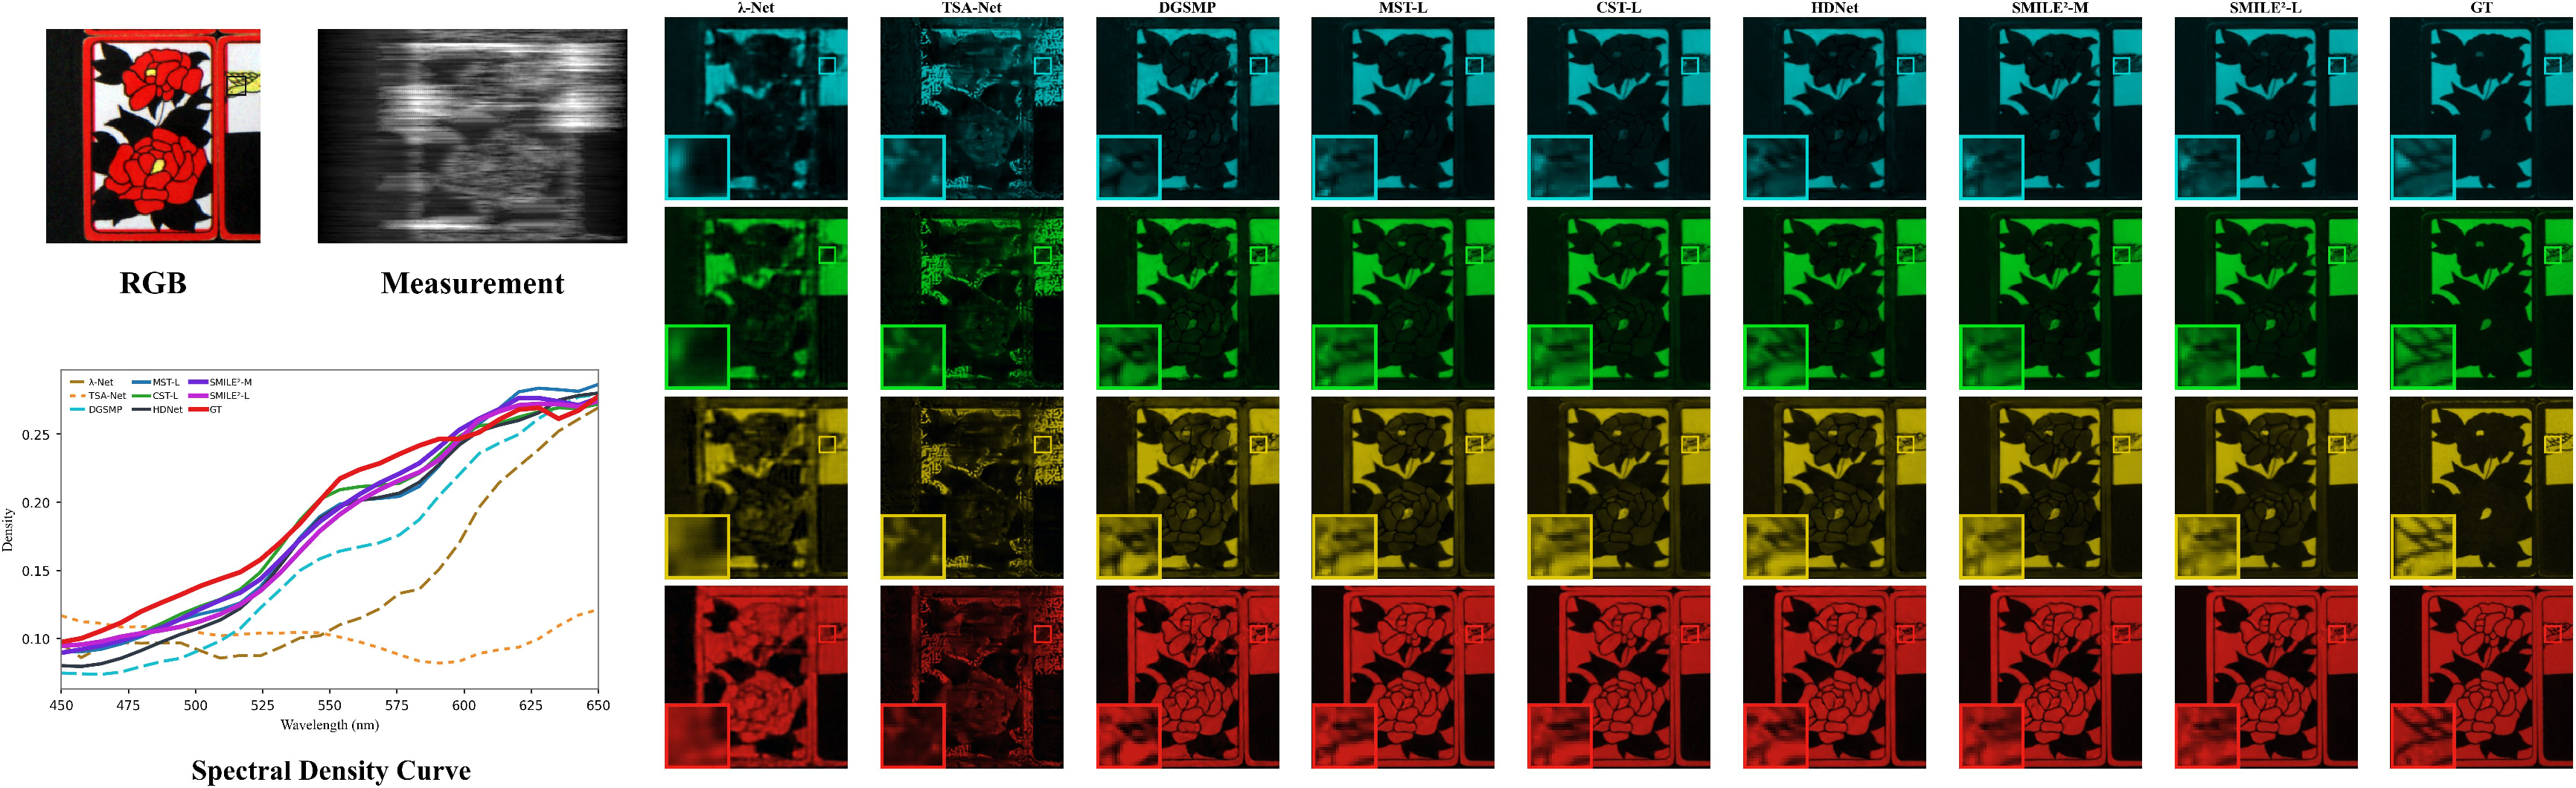
\includegraphics[width=\textwidth]{final/scene07_unified_layout.pdf}
  \caption{Simulation Scene 7. The same set of end-to-end comparison methods and curve styles are used as in Scene 5.}
  \label{fig:sota_simu_scene7}
\end{figure*}

Figures~\ref{fig:sota_simu_scene5} and \ref{fig:sota_simu_scene7} show representative simulation results.
Scene 5 contains weak text boundaries in the ``SIG'' region, where low-accuracy methods recover the rough layout but introduce artifacts and spectral distortions.
Transformer baselines are cleaner, yet local structures are still softened.
\smiletwo-M and \smiletwo-L preserve sharper letters and local textures, and their spectral density curves more closely follow the ground truth.
Scene 7 contains strong spatial--spectral contrast.
\smiletwo{} maintains clearer petal boundaries across multiple bands and suppresses dispersion-like artifacts.
Together with the SAM scores in Table~\ref{tab:sota_main}, these visual results indicate that the improvement is reflected not only in average image quality but also in spectral consistency and local structure.

\begin{figure*}[!t]
  \centering
  
\includegraphics[width=\textwidth]{final/real4_generalization_grid_256_hdnet_smilel.pdf}
  \caption{Real CASSI measurement results. Since real measurements do not provide ground-truth HSIs, we compare representative bands and zoomed local regions.}
  \label{fig:sota_real}
\end{figure*}

We also apply \smiletwo{} to real CASSI measurements.
As shown in Fig.~\ref{fig:sota_real}, \smiletwo{} produces stable reconstructions on real coded measurements.
Compared with other end-to-end baselines, it shows fewer artifacts in smooth regions and clearer local edges, suggesting that the estimation--evolution structure generalizes to real measurements.

\subsection{Ablation Study}

\begin{table}[!t]
\centering
\caption{Ablation study under the \smiletwo-S setting.}
\label{tab:ablation}
\scriptsize
\begin{adjustbox}{width=\columnwidth}
\begin{tabular}{llccc}
\toprule
ID & Variant & PSNR$\uparrow$ & SSIM$\uparrow$ & SAM$\downarrow$ \\
\midrule
B0 & \smiletwo-S & 35.9378 & 0.9557 & 0.1116 \\
A1 & w/o \sfestimator{} & 35.4985 & 0.9482 & 0.1352 \\
A2 & w/o \sfevolver{} & 24.3386 & 0.6160 & 0.4790 \\
A3 & w/o shifted-mask gating & 35.3727 & 0.9473 & 0.1517 \\
A4 & w/o \(\lambda\)-derivative & 35.5002 & 0.9484 & 0.1345 \\
\bottomrule
\end{tabular}
\end{adjustbox}
\end{table}

The ablation results show the contribution of the estimation--evolution decomposition.
Removing \sfestimator{} keeps the evolution structure but removes the initial-field correction from \(Q_0\) and \(H_0\odot M\), causing degradation in PSNR, SSIM, and SAM.
Removing \sfevolver{} forces the network to rely only on the estimated field and leads to severe quality loss, showing that structured evolution is not a simple post-processing branch.
Removing shifted-mask gating or the \(\lambda\)-derivative term also worsens SAM, indicating that mask-conditioned propagation and spectral propagation both contribute to spectral fidelity.

\subsection{Mechanism Analysis}

We further analyze whether \smiletwo{} actually exploits cross-band information.
We estimate an implicit cross-band mixing map through finite-difference impulse response and compare performance drops under equal-count occlusion of neighboring and distant bands.
As shown in Fig.~\ref{fig:mechanism}, the model exhibits strong diagonal responses, meaningful nearby-band coupling, and weak but non-negligible long-range spectral interactions.
This indicates that \smiletwo{} induces measurable cross-band propagation with both local spectral coupling and long-range spectral context.

\begin{figure*}[!t]
  \centering
  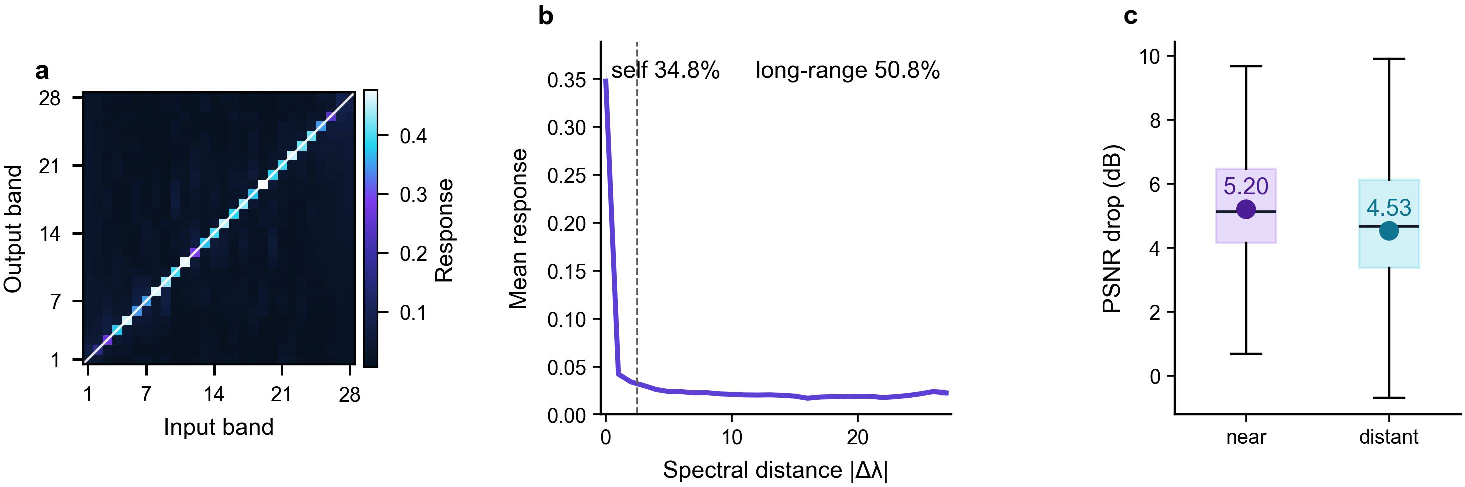
\includegraphics[width=\textwidth]{final/cross_band_mechanism_panel.pdf}
  \caption{Mechanism analysis of cross-band propagation. The finite-difference mixing map and equal-count occlusion results reveal how \smiletwo{} exploits spectral context.}
  \label{fig:mechanism}
\end{figure*}

\section{Discussion}

\paragraph{Interpretability of physical evolution.}
Unlike direct pairwise token interaction, \swp{} writes spatial--spectral mixing as Fourier-domain damped-wave propagation.
This gives explicit structural meaning to global propagation, the spectral second-derivative term, and CASSI mask gating.
The mechanism analysis further shows that the model uses both neighboring and distant spectral contexts, which is consistent with the coexistence of spectral continuity and material-dependent variation in HSIs.

\paragraph{Estimation before evolution.}
The CASSI shift-back field contains major scene structures but also contains mask modulation, dispersion overlap, and spectral aliasing.
Directly evolving \(H_0\) is therefore suboptimal.
\sfestimator{} uses \(Q_0\) and \(H_0\odot M\) to estimate a more reliable initial spectral field, allowing \sfevolver{} to focus on structured spatial--spectral propagation.
This decomposition makes measurement-consistent field estimation and physics-inspired field evolution complementary within a single-pass network.

\section{Conclusion}

We presented \smiletwo{}, a single-pass spectral-field estimation--evolution framework for CASSI reconstruction.
\smiletwo{} constructs measurement-aware CASSI fields, estimates a cleaner initial spectral field, and evolves it through a Fourier-domain damped-wave propagator.
Experiments on simulation and real CASSI measurements demonstrate state-of-the-art end-to-end reconstruction quality with compact computation.
Mechanism analyses further show that \smiletwo{} exploits structured cross-band propagation, providing a physically motivated alternative to generic token mixing for hyperspectral reconstruction.

\section{Additional Diagnostics}

\subsection{Inference Latency and Peak Memory}

Table~\ref{tab:runtime_memory_appendix} reports inference latency and peak allocated memory under the same test protocol.
All methods are tested scene-by-scene at \(256\times256\times28\) resolution.
These measurements complement FLOPs and parameter counts, since actual throughput also depends on kernel implementation, memory access, and FFT scheduling.

\begin{table}[!t]
\centering
\caption{Inference latency and peak allocated memory on the TSA simulation benchmark.}
\label{tab:runtime_memory_appendix}
\scriptsize
\begin{adjustbox}{width=\columnwidth}
\begin{tabular}{lccccc}
\toprule
Method & Params & GFLOPs & Time & Alloc. & Reserved \\
 & (M) & (G) & (ms) & (MB) & (MB) \\
\midrule
GAP-TV & 4.27 & 75.63 & 38.23 & 156.17 & 194.00 \\
\(\lambda\)-Net & 32.73 & 28.40 & 19.71 & 414.00 & 500.00 \\
TSA-Net & 44.25 & 73.83 & 60.47 & 635.97 & 784.00 \\
DGSMP & 3.76 & 646.36 & 86.89 & 658.29 & 774.00 \\
MST-L & 2.02 & 25.67 & 84.96 & 158.76 & 274.00 \\
CST-L & 3.00 & 20.34 & 38.25 & 316.45 & 388.00 \\
HDNet & 2.37 & 154.73 & 13.49 & 134.94 & 178.00 \\
\midrule
\smiletwo-S & 1.02 & 28.28 & 40.26 & 236.47 & 274.00 \\
\smiletwo-M & 2.00 & 28.28 & 39.16 & 251.79 & 290.00 \\
\smiletwo-L & 3.23 & 38.60 & 57.82 & 278.42 & 316.00 \\
\bottomrule
\end{tabular}
\end{adjustbox}
\end{table}

\begin{figure}[!t]
  \centering
  
\includegraphics[width=\columnwidth]{final/appendix_runtime_memory.pdf}
  \caption{Latency and peak-memory comparison under the same test protocol.}
  \label{fig:runtime_memory_appendix}
\end{figure}

\subsection{Learned SWP Parameter Profiles}

Figure~\ref{fig:swp_param_appendix} visualizes the learned \swp{} parameters in \smiletwo-M.
\(\alpha(f_\lambda)\) and \(v_s(f_\lambda)\) are computed from 28-mode \swp{} layers and thus correspond to spectral-mode-dependent damping and propagation speed.
\(v_\lambda\) and \(t\) are module-level learnable scalars that control spectral second-derivative strength and evolution depth.
Figure~\ref{fig:swp_kernel_appendix} further derives 3D damped-wave kernel visualizations from the learned average parameters under different evolution depths.

\begin{figure}[!t]
  \centering
  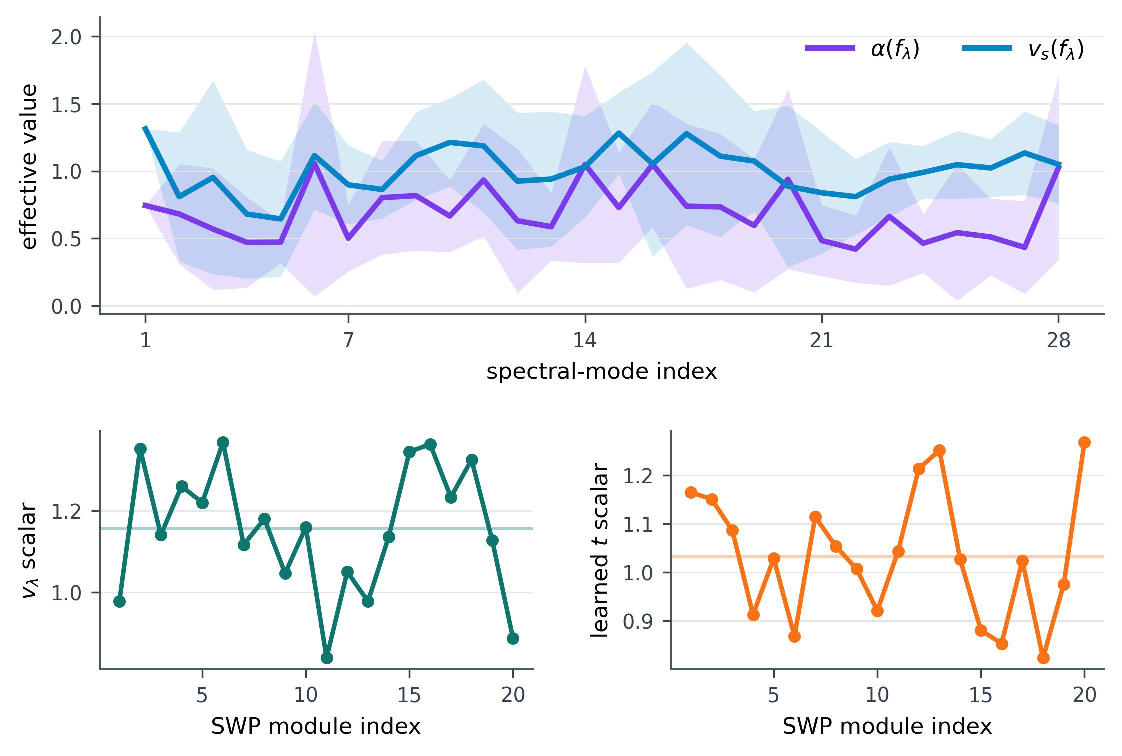
\includegraphics[width=\columnwidth]{final/appendix_smile_m_swp_profiles.pdf}
  \caption{Learned spectral-mode parameters in \smiletwo-M.}
  \label{fig:swp_param_appendix}
\end{figure}

\begin{figure}[!t]
  \centering
  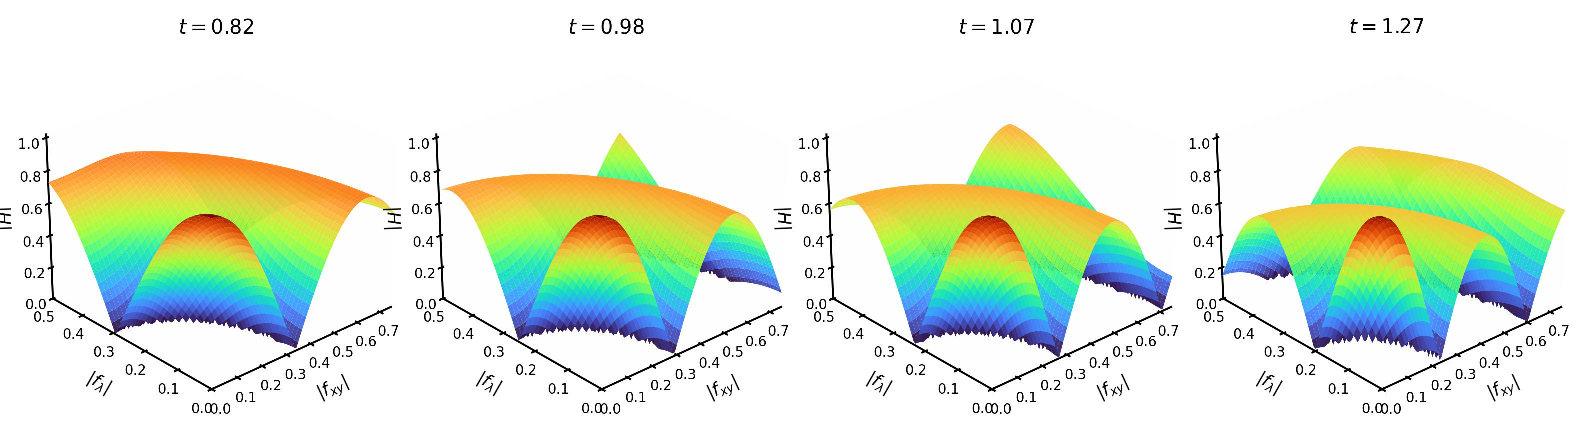
\includegraphics[width=\columnwidth]{final/appendix_smile_m_wave_kernel_3d_by_t.pdf}
  \caption{Derived 3D visualization of the learned damped-wave kernel under different evolution depths \(t\).}
  \label{fig:swp_kernel_appendix}
\end{figure}

\bibliography{smile2_aaai2026}

\end{document}










